
\de{ĐỀ THI HỌC KỲ I NĂM HỌC 2022-2023}{THPT Chuyên Nguyễn Thất Thành - Yên Bái}
\begin{center}
	\textbf{PHẦN 1 - TRẮC NGHIỆM}
\end{center}
\Opensolutionfile{ans}[ans/ans]
%%=====Câu 1
\begin{ex}%[0H2Y3-1]%[Dự án đề kiểm tra HKI NH22-23- Thầy Hóa]%[THPT Chuyên Nguyễn Tất Thành]
Cho tam giác $ABC$. Gọi $M$, $N$ lần lượt là trung điểm của $AB$, $AC$. Mệnh đề nào sau đây đúng?
\choice
{$\vec{MN}=-\dfrac{1}{2}\vec{BC}$}
{\True $\vec{MN}=\dfrac{1}{2}\vec{BC}$}
{$\vec{MN}=-2\vec{BC}$}
{$\vec{MN}=2\vec{BC}$}
\loigiai{
\immini{
Vì $MN$ là đường trung bình của $\triangle ABC$ nên $\vec{MN}=\dfrac{1}{2}\vec{BC}$.
}{
\begin{tikzpicture}[>=stealth,line join=round,line cap=round,font=\footnotesize,scale=1]
	\def\a{4};
	\def\b{3};
	\def\g{70};
	\path
	(0,0) coordinate (B)
	(0:\a) coordinate (C)
	(\g:\b) coordinate (A)
	($(A)!0.5!(B)$) coordinate (M)
	($(A)!0.5!(C)$) coordinate (N)
	;
	\draw
	(A)--(B)--(C)--cycle (M)--(N)
	;
	\foreach \x/\g in {B/-135,C/-45,A/90,M/135,N/45}\fill[black](\x) circle (1pt) +(\g:3mm) node {$\x$};
	\foreach \x/\y in {A/M,M/B}{\node[rotate=30] at ($(\x)!0.5!(\y)$){|};}
	\foreach \x/\y in {A/N,N/C}{\node[rotate=-10] at ($(\x)!0.5!(\y)$){$\parallel$};}
\end{tikzpicture}
}
}
\end{ex}

%%=====Câu 2
\begin{ex}%[0X1Y1-4]%[Dự án đề kiểm tra HKI NH22-23- Thầy Hóa]%[THPT Chuyên Nguyễn Tất Thành]
Người ta đo chiều dài một cây cầu được $996$ m với độ chính xác là $0{,}5$ m. Chiều dài thực của cây cầu đó thuộc đoạn nào sau đây?
\choice
{$[996;996{,}5]$}
{$[995;997]$}
{\True $[995{,}5;996{,}5]$}
{$[995{,}5;996]$}
\loigiai{
Chiều dài thực của cây cầu đó thuộc đoạn $[995{,}5;996{,}5]$.
}
\end{ex}

%%=====Câu 3
\begin{ex}%[0X1B3-1]%[Dự án đề kiểm tra HKI NH22-23- Thầy Hóa]%[THPT Chuyên Nguyễn Tất Thành]
Điểm thi tuyển sinh vào lớp $10$ ba môn Toán, Văn, Tiếng Anh của một học sinh lần lượt là $9{,}0$; $8{,}5$; $8{,}0$. Điểm thi trung bình ba môn thi của học sinh đó là
\choice
{$8{,}0$}
{$7{,}5$}
{$25{,}5$}
{\True $8{,}5$}
\loigiai{
Điểm thi trung bình ba môn thi của học sinh đó là
\[(9{,}0+8{,}5+8{,}0):3=8{,}5. \]
}
\end{ex}

%%=====Câu 4
\begin{ex}%[0D2B1-2]%[Dự án đề kiểm tra HKI NH22-23- Thầy Hóa]%[THPT Chuyên Nguyễn Tất Thành]
Miền nghiệm của bất phương trình $x+y\leq 2$ (phần không bị gạch) được biểu diễn bởi hình vẽ nào dưới đây?
\choice
{\begin{tikzpicture}[>=stealth,scale=0.5]
		\def\a{1}
		\def\b{2}
		\fill[pattern=north east lines] (-3,-1)--(-3,3)--(1,3)--cycle;
		\draw[->] (-3,0) -- (2,0) node[below] {\scriptsize $x$};
		\draw[->] (0,-1) -- (0,3) node[above left] {\scriptsize $y$};
		\clip (-3,-1)rectangle(2,3);
		\draw[thick,samples=150,smooth,domain=-3:2] plot(\x,{\a*\x+(\b)});
		\fill (0,0) circle (1.5pt) node[below left]{\scriptsize $O$};
		\fill (-2,0) circle (1.5pt) node[below]{\scriptsize $-2$};
		\fill (0,2) circle (1.5pt) node[below right]{\scriptsize $2$};
\end{tikzpicture}}
{\begin{tikzpicture}[>=stealth,scale=0.5]
		\def\a{-1}
		\def\b{2}
		\fill[pattern=north east lines] (-1,3)--(-2,3)--(-2,-1)--(3,-1)--cycle;
		\draw[->] (-2,0) -- (3,0) node[below] {\scriptsize $x$};
		\draw[->] (0,-1) -- (0,3) node[left] {\scriptsize $y$};
		\clip (-2,-1)rectangle(3,3);
		\draw[thick,samples=150,smooth,domain=-2:3] plot(\x,{\a*\x+(\b)});
		\fill (0,0) circle (1.5pt) node[below left]{\scriptsize $O$};
		\fill (2,0) circle (1.5pt) node[above]{\scriptsize $2$};
		\fill (0,2) circle (1.5pt) node[above right]{\scriptsize $2$};
\end{tikzpicture}}
{\begin{tikzpicture}[>=stealth,scale=0.5]
		\def\a{1}
		\def\b{2}
		\fill[pattern=north east lines] (-3,-1)--(2,-1)--(2,3)--(1,3)--cycle;
		\draw[->] (-3,0) -- (2,0) node[below] {\scriptsize $x$};
		\draw[->] (0,-1) -- (0,3) node[left] {\scriptsize $y$};
		\clip (-3,-1)rectangle(2,3);
		\draw[thick,samples=150,smooth,domain=-3:2] plot(\x,{\a*\x+(\b)});
		\fill (0,0) circle (1.5pt) node[below left]{\scriptsize $O$};
		\fill (-2,0) circle (1.5pt) node[above left]{\scriptsize $-2$};
		\fill (0,2) circle (1.5pt) node[above left]{\scriptsize $2$};
\end{tikzpicture}}
{\True \begin{tikzpicture}[>=stealth,scale=0.5]
		\def\a{-1}
		\def\b{2}
		\fill[pattern=north east lines] (-1,3)--(3,3)--(3,-1)--cycle;
		\draw[->] (-2,0) -- (3,0) node[below right] {\scriptsize $x$};
		\draw[->] (0,-1) -- (0,3) node[above left] {\scriptsize $y$};
		\clip (-2,-1)rectangle(3,3);
		\draw[thick,samples=150,smooth,domain=-2:3] plot(\x,{\a*\x+(\b)});
		\fill (0,0) circle (1.5pt) node[below left]{\scriptsize $O$};
		\fill (2,0) circle (1.5pt) node[below]{\scriptsize $2$};
		\fill (0,2) circle (1.5pt) node[below left]{\scriptsize $2$};
\end{tikzpicture}}
\loigiai{
Miền nghiệm của bất phương trình $x+y\leq 2$ chứa đường thẳng $x+y=2$ và điểm $O(0,0)$.
}
\end{ex}

%%=====Câu 5
\begin{ex}%[0D2B2-2]%[Dự án đề kiểm tra HKI NH22-23- Thầy Hóa]%[THPT Chuyên Nguyễn Tất Thành]
\immini{
Miền không bị gạch chéo trong hình vẽ bên biểu diễn miền nghiệm của hệ bất phương trình nào dưới đây?
\choice
{$\heva{&x+y-1\geq 0\\&2x-y+4<0}$}
{\True $\heva{&x+y-1\leq 0\\&2x-y+4\geq 0}$}
{$\heva{&x+y-1\leq 0\\&2x-y+4<0}$}
{$\heva{&x+y-1\geq 0\\&2x-y+4\leq 0}$}
}{
\begin{tikzpicture}[>=stealth,scale=0.75]
	\def\a{2}
	\def\b{4}
	\fill[pattern=north east lines] (-3,-2)--(-4,-2)--(-4,5)--(4,5)--(4,-2)--(3,-2)--(-1,2)--cycle;
	\draw[->] (-4,0) -- (4,0) node[below] {\scriptsize $x$};
	\draw[->] (0,-2) -- (0,5) node[left] {\scriptsize $y$};
	\clip (-4,-2)rectangle(4,5);
	\draw[thick,samples=150,smooth,domain=-4:4] plot(\x,{\a*\x+(\b)});
	\draw[thick,samples=150,smooth,domain=-4:4] plot(\x,{-1*\x+1});
	\foreach \x in {-3,-2,-1,1,2,3}{\draw (\x,0.1)--++(-90:0.2)node[below]{\scriptsize $\x$};}
	\foreach \y in {-1,1,2,3,4}{\draw (-0.1,\y)--++(0:0.2)node[right]{\scriptsize $\y$};}
	\fill (0,0) circle (1.5pt) node[below left]{\scriptsize $O$};
\end{tikzpicture}
}
\loigiai{
Miền nghiệm của hệ bất phương trình có chứa gốc tọa độ $O(0,0)$ nên loại các hệ bất phương trình $\heva{&x+y-1\geq 0\\&2x-y+4<0}$; $\heva{&x+y-1\leq 0\\&2x-y+4<0}$ và $\heva{&x+y-1\geq 0\\&2x-y+4\leq 0}$.\\

}
\end{ex}

%%=====Câu 6
\begin{ex}%[0H1Y2-2]%[Dự án đề kiểm tra HKI NH22-23- Thầy Hóa]%[THPT Chuyên Nguyễn Tất Thành]
Cho tam giác $ABC$ có $BC=a$, $CA=b$, $AB=c$ và $R$ là bán kính đường tròn ngoại tiếp tam giác $ABC$. Mệnh đề nào sau đây \textbf{sai}?
\choice
{$\sin C=\dfrac{c\cdot \sin A}{a}$}
{\True $a=2R\cdot\cos A$}
{$a=\dfrac{b\cdot\sin A}{\sin B}$}
{$b=2R\cdot\sin B$}
\loigiai{
Theo định lý $\sin$, ta có $\dfrac{a}{\sin A}=\dfrac{b}{\sin B}=\dfrac{c}{\sin C}=2R$ nên khẳng định  $a=2R\cdot\cos A$ là sai.
}
\end{ex}

%%=====Câu 7
\begin{ex}%[0H2Y1-2]%[Dự án đề kiểm tra HKI NH22-23- Thầy Hóa]%[THPT Chuyên Nguyễn Tất Thành]
Cho hình bình hành $ABCD$ tâm $O$. Véc-tơ cùng hướng với $\vec{BO}$ là
\choice
{$\vec{AO}$}
{$\vec{DO}$}
{\True $\vec{OD}$}
{$\vec{CO}$}
\loigiai{
\immini{
Véc-tơ cùng hướng với $\vec{BO}$ là $\vec{OD}$.
}{
\begin{tikzpicture}[>=stealth,line join=round,line cap=round,font=\footnotesize,scale=1]
	\def\a{4};
	\def\b{1.5};
	\def\g{50};
	\path
	(0,0) coordinate (D)
	(0:\a) coordinate (C)
	(\g:\b) coordinate (A)
	($(A)+(C)-(D)$) coordinate (B)
	(intersection of A--C and B--D) coordinate (O)
	;
	\draw
	(A)--(B)--(C)--(D)--cycle (A)--(C) (B)--(D)
	;
	\foreach \x/\g in {A/135,B/45,C/-45,D/-135,O/-90}\fill[black](\x) circle (1pt) +(\g:3mm) node {$\x$};
\end{tikzpicture}
}
}
\end{ex}

%%=====Câu 8
\begin{ex}%[0D2Y2-1]%[Dự án đề kiểm tra HKI NH22-23- Thầy Hóa]%[THPT Chuyên Nguyễn Tất Thành]
Hệ bất phương trình nào sau đây là hệ bất phương trình bậc nhất hai ẩn?
\choice
{\True $\heva{&x-3y>0\\&x+y>3}$}
{$\heva{&2x-3y\geq 0\\&x+\sqrt{y}<3}$}
{$\heva{&2x-3y\geq 0\\&x+y^2<3}$}
{$\heva{&2x^2-3y\geq 0\\&x+y<3}$}
\loigiai{
Hệ bất phương trình $\heva{&x-3y>0\\&x+y>3}$ là hệ bất phương trình bậc nhất hai ẩn.
}
\end{ex}

%%=====Câu 9
\begin{ex}%[0H1B2-2]%[Dự án đề kiểm tra HKI NH22-23- Thầy Hóa]%[THPT Chuyên Nguyễn Tất Thành]
Cho tam giác $ABC$ có $\widehat{B}=10^\circ$, $\widehat{C}=20^\circ$, $AB=10$, $AC=12$. Tính diện tích tam giác $ABC$.
\choice
{$S_{\triangle ABC}=60$}
{\True $S_{\triangle ABC}=30$}
{$S_{\triangle ABC}=40$}
{$S_{\triangle ABC}=20$}
\loigiai{
Ta có $\widehat{A}=180^\circ-\left(\widehat{B}+\widehat{C}\right)=180^\circ-\left(10^\circ+20^\circ\right)=150^\circ$.\\
Diện tích tam giác $ABC$: $S_{\triangle ABC}=\dfrac{1}{2}AB\cdot AC\cdot\sin A=\dfrac{1}{2}\cdot 10\cdot 12\cdot \sin 150^\circ=30$.
}
\end{ex}

%%=====Câu 10
\begin{ex}%[0H1Y2-1]%[Dự án đề kiểm tra HKI NH22-23- Thầy Hóa]%[THPT Chuyên Nguyễn Tất Thành]
Cho tam giác $ABC$ có $BC=a$, $CA=b$, $AB=c$. Mệnh đề nào sau đây đúng?
\choice
{$\cos B=\dfrac{a^2+c^2-b^2}{2ab}$}
{$\cos B=\dfrac{c^2+b^2-a^2}{2cb}$}
{\True $\cos B=\dfrac{a^2+c^2-b^2}{2ac}$}
{$\cos B=\dfrac{a^2+b^2-c^2}{2ab}$}
\loigiai{
Theo hệ quả của định lý cô-sin thì khẳng định $\cos B=\dfrac{a^2+c^2-b^2}{2ac}$ là đúng.
}
\end{ex}

%%=====Câu 11
\begin{ex}%[0H1Y1-2]%[Dự án đề kiểm tra HKI NH22-23- Thầy Hóa]%[THPT Chuyên Nguyễn Tất Thành]
Trong các đẳng thức sau đây, đẳng thức nào đúng?
\choice
{$\sin \left(180^\circ-\alpha\right)=-\sin \alpha$}
{$\cot \left(180^\circ-\alpha\right)=\cot \alpha\ \left(0^\circ>\alpha<180^\circ\right)$}
{$\cos \left(180^\circ-\alpha\right)=\cos \alpha$}
{\True $\tan \left(180^\circ-\alpha\right)=-\tan \alpha\ \left(\alpha\neq 90^\circ\right)$}
\loigiai{
Khẳng định $\tan \left(180^\circ-\alpha\right)=-\tan \alpha\ \left(\alpha\neq 90^\circ\right)$ là đúng.
}
\end{ex}

%%=====Câu 12
\begin{ex}%[0X1Y1-1]%[Dự án đề kiểm tra HKI NH22-23- Thầy Hóa]%[THPT Chuyên Nguyễn Tất Thành]
Cho $a$ là số gần đúng của số $\overline{a}$. Sai số tuyệt đối của số gần đúng $\overline{a}$ là
\choice
{\True $\Delta_a=\left|a-\overline{a}\right|$}
{$\Delta_a=a-\overline{a}$}
{$\Delta_a=a+\overline{a}$}
{$\Delta_a=\left|a+\overline{a}\right|$}
\loigiai{
Sai số tuyệt đối của số gần đúng $\overline{a}$ là $\Delta_a=\left|a-\overline{a}\right|$.
}
\end{ex}

%%=====Câu 13
\begin{ex}%[0X1B3-2]%[Dự án đề kiểm tra HKI NH22-23- Thầy Hóa]%[THPT Chuyên Nguyễn Tất Thành]
Giá của một số loại túi xách (đơn vị nghìn đồng) được cho như sau:
\[350\quad 300\quad 650\quad 300\quad 450\quad 500\quad 300\quad 250\quad 400. \]
Tìm số trung vị của mẫu số liệu trên.
\choice
{$300$}
{$450$}
{$400$}
{\True $350$}
\loigiai{
Mẫu số liệu được sắp xếp theo thứ tự tăng dần như sau
\[250\quad 300\quad 300\quad 300\quad 350\quad 400\quad 450\quad 500\quad 650. \]
Do đó số trung vị của mẫu số liệu là $350$.
}
\end{ex}

%%=====Câu 14
\begin{ex}%[0H2B2-1]%[Dự án đề kiểm tra HKI NH22-23- Thầy Hóa]%[THPT Chuyên Nguyễn Tất Thành]
Cho hình bình hành $ABCD$. Gọi $M$ và $N$ lần lượt là trung điểm của đoạn $BC$ và $AD$. Khi đó $\vec{NC}+\vec{MC}$ bằng
\choice
{$\vec{MN}$}
{$\vec{CA}$}
{$\vec{NM}$}
{\True $\vec{AC}$}
\loigiai{
\immini{
Ta có $\begin{aligned}[t]
	\vec{NC}+\vec{MC}&=\vec{NA}+\vec{AC}+\vec{MC}\\
	&=\vec{MB}+\vec{MC}+\vec{AC}\\
	&=\vec{0}+\vec{AC}\\
	&=\vec{AC}.
\end{aligned}$
}{
\begin{tikzpicture}[>=stealth,line join=round,line cap=round,font=\footnotesize,scale=1]
	\def\a{4};
	\def\b{1.5};
	\def\g{50};
	\path
	(0,0) coordinate (D)
	(0:\a) coordinate (C)
	(\g:\b) coordinate (A)
	($(A)+(C)-(D)$) coordinate (B)
	($(B)!0.5!(C)$) coordinate (M)
	($(A)!0.5!(D)$) coordinate (N)
	;
	\draw
	(A)--(B)--(C)--(D)--cycle
	;
	\foreach \x/\g in {A/135,B/45,C/-45,D/-135,M/0,N/180}\fill[black](\x) circle (1pt) +(\g:3mm) node {$\x$};
	\foreach \x/\y in {A/N,N/D,M/C,M/B}{\node[rotate=30] at ($(\x)!0.5!(\y)$){|};}
\end{tikzpicture}
}
}
\end{ex}

%%=====Câu 15
\begin{ex}%[0H4Y1-7]%[Dự án đề kiểm tra HKI NH22-23- Thầy Hóa]%[THPT Chuyên Nguyễn Tất Thành]
Trong hệ tọa độ $Oxy$ cho $\triangle ABC$ có $A(1;2)$, $B(4;6)$, $C(7;-2)$. Tọa độ trọng tâm $G$ của $\triangle ABC$ là
\choice
{$G(8;4)$}
{\True $G(4;2)$}
{$G(2;4)$}
{$G\left(4;\dfrac{10}{3}\right)$}
\loigiai{
Ta có $\heva{&x_G=\dfrac{1+4+7}{3}=4\\&y_G=\dfrac{2+6+(-2)}{3}=2.}$\\
Vậy tọa độ trọng tâm $G$ của $\triangle ABC$ là $G(4;2)$.
}
\end{ex}

%%=====Câu 16
\begin{ex}%[0D2B2-2]%[Dự án đề kiểm tra HKI NH22-23- Thầy Hóa]%[THPT Chuyên Nguyễn Tất Thành]
Cho hệ bất phương trình $\heva{&x+3y\geq 2\\&2x+y\leq -1}$. Điểm nào sau đây thuộc miền nghiệm của hệ bất phương trình đã cho?
\choice
{$(-1;0)$}
{$(1;3)$}
{$(0;1)$}
{\True $(-1;1)$}
\loigiai{
\begin{itemize}
	\item Thế $x=-1$, $y=0$ vào bất phương trình $x+3y\geq 2$ thì không thỏa mãn.
	\item Thế $x=1$, $y=3$ vào bất phương trình $2x+y\leq 1$ thì không thỏa mãn.
	\item Thế $x=0$, $y=1$ vào bất phương trình $x+3y\geq 2$ thì không thỏa mãn.
	\item Thế $x=-1$, $y=1$ vào hệ bất phương trình $\heva{&x+3y\geq 2\\&2x+y\leq -1}$, ta thấy thỏa mãn.
\end{itemize}
}
\end{ex}

%%=====Câu 17
\begin{ex}%[0X1B3-4]%[Dự án đề kiểm tra HKI NH22-23- Thầy Hóa]%[THPT Chuyên Nguyễn Tất Thành]
Một cửa hàng thống kê cỡ giày của một số khách hàng nam được chọn ngẫu nhiên cho kết quả như sau:
\[37\quad 38\quad 38\quad 39\quad 40\quad 40\quad 39\quad 40\quad 41\quad 40\quad 37\quad 40. \]
Mốt của số liệu trên là
\choice
{$41$}
{$38$}
{$39$}
{\True $40$}
\loigiai{
Bảng tần số của dãy số liệu trên
\begin{center}
	\begin{tabular}{|c|c|c|c|c|c|c|}
	\hline
	Giá trị $(x)$ &$37$ &$38$ &$39$ &$40$ &$41$ &\\
	\hline
	Tân số $(n)$ &$2$ &$2$ &$2$ &$5$ &$1$ &$N=12$\\
	\hline 
	\end{tabular}
\end{center}
Mốt của số liệu trên là $40$.
}
\end{ex}

%%=====Câu 18
\begin{ex}%[0H3Y1-3]%[Dự án đề kiểm tra HKI NH22-23- Thầy Hóa]%[THPT Chuyên Nguyễn Tất Thành]
Trong mặt phẳng tọa độ $Oxy$ cho $\vec{u}=-2\vec{i}+3\vec{j}$. Tìm tọa độ $\vec{u}$.
\choice
{$\vec{u}=\left(-2\vec{i};3\vec{j}\right)$}
{$\vec{u}=\left(2;-3\right)$}
{\True $\vec{u}=\left(-2;3\right)$}
{$\vec{u}=\left(3;-2\right)$}
\loigiai{
Ta có $\vec{u}=\left(-2;3\right)$.
}
\end{ex}

%%=====Câu 19
\begin{ex}%[0X1Y1-1]%[Dự án đề kiểm tra HKI NH22-23- Thầy Hóa]%[THPT Chuyên Nguyễn Tất Thành]
Cho $\Delta_a$ là sai số tuyệt đối của số gần đúng $a$. Sai số tương đối của số gần đúng $a$ là
\choice
{$\delta_a=\dfrac{|a|}{\Delta_a}$}
{$\delta_a=\dfrac{a}{\Delta_a}$}
{\True $\delta_a=\dfrac{\Delta_a}{|a|}$}
{$\delta_a=\dfrac{\Delta_a}{a}$}
\loigiai{
Sai số tương đối của số gần đúng $a$ là $\delta_a=\dfrac{\Delta_a}{|a|}$.
}
\end{ex}

%%=====Câu 20
\begin{ex}%[0H1Y2-2]%[Dự án đề kiểm tra HKI NH22-23- Thầy Hóa]%[THPT Chuyên Nguyễn Tất Thành]
Cho tam giác $ABC$ có $BC=a$, $CA=b$, $AB=c$. Diện tích của tam giác $ABC$ là
\choice
{$S=\dfrac{1}{2}bc\sin C$}
{$S=\dfrac{1}{2}bc\sin B$}
{$S=\dfrac{1}{2}ca\sin A$}
{\True $S=\dfrac{1}{2}bc\sin A$}
\loigiai{
Diện tích của tam giác $ABC$ là $S=\dfrac{1}{2}bc\sin A$.
}
\end{ex}

%%=====Câu 21
\begin{ex}%[0H3B1-3]%[Dự án đề kiểm tra HKI NH22-23- Thầy Hóa]%[THPT Chuyên Nguyễn Tất Thành]
Trong mặt phẳng tọa độ $Oxy$ cho hai điểm $M(-3;1)$ và $N(6;-4)$. Tìm tọa độ của $\vec{MN}$.
\choice
{\True $\vec{MN}=(9;-5)$}
{$\vec{MN}=(-9;-5)$}
{$\vec{MN}=(-9;5)$}
{$\vec{MN}=(9;5)$}
\loigiai{
Ta có $\vec{MN}=(9;-5)$.
}
\end{ex}

%%=====Câu 22
\begin{ex}%[0H1B1-3]%[Dự án đề kiểm tra HKI NH22-23- Thầy Hóa]%[THPT Chuyên Nguyễn Tất Thành]
Giá trị của biểu thức $T=\cos 60^\circ\cdot \sin 30^\circ+\cos^2 30^\circ$ bằng
\choice
{$\dfrac{1}{2}$}
{$0$}
{\True $1$}
{$\dfrac{1+2\sqrt{3}}{4}$}
\loigiai{
Ta có $T=\cos 60^\circ\cdot \sin 30^\circ+\cos^2 30^\circ=\dfrac{1}{2}\cdot \dfrac{1}{2}+\left(\dfrac{\sqrt{3}}{2}\right)^2=\dfrac{1}{4}+\dfrac{3}{4}=1$.
}
\end{ex}

%%=====Câu 23
\begin{ex}%[0H1B2-1]%[Dự án đề kiểm tra HKI NH22-23- Thầy Hóa]%[THPT Chuyên Nguyễn Tất Thành]
Cho tam giác $ABC$ có $\widehat{A}=135^\circ$, $AB=2\sqrt{2}$, $AC=3$. Độ dài cạnh $BC$ bằng
\choice
{$\sqrt{17-6\sqrt{6}}$}
{$\sqrt{5}$}
{\True $\sqrt{29}$}
{$\sqrt{17+6\sqrt{6}}$}
\loigiai{
Áp dụng định lý cô-sin, ta có
\allowdisplaybreaks
\begin{eqnarray*}
BC^2&=&AB^2+AC^2-2AB\cdot AC\cdot \cos A\\
&=&\left(2\sqrt{2}\right)^2+3^2-2\cdot 2\sqrt{2}\cdot 3\cdot\cos 135^\circ\\
&=&29.
\end{eqnarray*}
Suy ra $BC=\sqrt{29}$.
}
\end{ex}

%%=====Câu 24
\begin{ex}%[0H3B1-3]%[Dự án đề kiểm tra HKI NH22-23- Thầy Hóa]%[THPT Chuyên Nguyễn Tất Thành]
Trong hệ tọa độ $Oxy$ cho $M(-3;1)$, $N(2;-3)$. Khoảng cách giữa hai điểm $M$, $N$ là
\choice
{$\sqrt{29}$}
{$3$}
{$5$}
{\True $\sqrt{41}$}
\loigiai{
Ta có $\vec{MN}=(5;-4)$.\\ Suy ra $MN=\sqrt{5^2+(-4)^2}=\sqrt{41}$.
}
\end{ex}

%%=====Câu 25
\begin{ex}%[0X1B3-3]%[Dự án đề kiểm tra HKI NH22-23- Thầy Hóa]%[THPT Chuyên Nguyễn Tất Thành]
Tứ phân vị thứ ba của mẫu số liệu
\[8\quad 7\quad 22\quad 20\quad 18\quad 15\quad 19\quad 11\quad 13 \]
là
\choice
{\True $Q_3=19{,}5$}
{$Q_3=18{,}5$}
{$Q_3=19$}
{$Q_3=20$}
\loigiai{
Mẫu số liệu được sắp xếp theo thứ tự như sau
\[7\quad 8\quad 11\quad 13\quad 15\quad 18\quad 19\quad 20\quad 22. \]
Tứ phân vị thứ ba của mẫu số liệu là $Q_3=\dfrac{19+20}{2}=19{,}5$.
}
\end{ex}

%%=====Câu 26
\begin{ex}%[0H2Y3-5]%[Dự án đề kiểm tra HKI NH22-23- Thầy Hóa]%[THPT Chuyên Nguyễn Tất Thành]
Cho tam giác $ABC$. Gọi $M$ là trung điểm của $BC$ và $G$ là trọng tâm của tam giác $ABC$. Đẳng thức nào sau đây đúng?
\choice
{$\vec{AB}+\vec{AC}=2\vec{AG}$}
{$\vec{AB}+\vec{AC}=2\vec{GM}$}
{$\vec{AB}+\vec{AC}=\dfrac{3}{2}\vec{AG}$}
{\True $\vec{AB}+\vec{AC}=2\vec{AM}$}
\loigiai{
\immini{
Ta có $\vec{AB}+\vec{AC}=2\vec{AM}$ (tính chất trung điểm).
}{
\begin{tikzpicture}[>=stealth,line join=round,line cap=round,font=\footnotesize,scale=1]
	\def\a{4};
	\def\b{3};
	\def\g{70};
	\path
	(0,0) coordinate (B)
	(0:\a) coordinate (C)
	(\g:\b) coordinate (A)
	($(B)!0.5!(C)$) coordinate (M)
	($(A)!0.5!(C)$) coordinate (N)
	(intersection of B--N and A--M) coordinate (G)
	;
	\draw
	(A)--(B)--(C)--cycle (A)--(M) (B)--(N)
	;
	\foreach \x/\g in {B/-135,C/-45,A/90,M/-90,G/180,N/10}\fill[black](\x) circle (1pt) +(\g:3mm) node {$\x$};
	\foreach \x/\y in {C/M,M/B}{\node[rotate=30] at ($(\x)!0.5!(\y)$){|};}
	\foreach \x/\y in {A/N,N/C}{\node[rotate=-10] at ($(\x)!0.5!(\y)$){$\parallel$};}
\end{tikzpicture}
}
}
\end{ex}

%%=====Câu 27
\begin{ex}%[0X1B4-1]%[Dự án đề kiểm tra HKI NH22-23- Thầy Hóa]%[THPT Chuyên Nguyễn Tất Thành]
Kết quả dự báo nhiệt độ cao nhất trong $10$ ngày cuối tháng $12$ năm $2022$ ở Yên Bái thu được như sau:
\[20\quad 21\quad 20\quad 19\quad 22\quad 17\quad 18\quad 18\quad 14\quad 16\ \left(^\circ \mathrm{C}\right). \]
Khoảng biến thiên $R$ của mẫu số liệu trên là
\choice
{\True $R=8$}
{$R=7$}
{$R=6$}
{$R=5$}
\loigiai{
Mẫu số liệu được sắp xếp theo thứ tự tăng dần như sau:
\[14\quad 16\quad 17\quad 18\quad 18\quad 19\quad 20\quad 20\quad 21\quad 22\ \left(^\circ \mathrm{C}\right). \]
Khoảng biến thiên $R$ của mẫu số liệu trên là
\[R=22-14=8. \]
}
\end{ex}

%%=====Câu 28
\begin{ex}%[0X1Y1-3]%[Dự án đề kiểm tra HKI NH22-23- Thầy Hóa]%[THPT Chuyên Nguyễn Tất Thành]
Làm tròn số $8315{,}456$ đến hàng chục, ta được số nào sau đây?
\choice
{$8315{,}5$}
{\True $8320$}
{$8310$}
{$8315$}
\loigiai{

}
\end{ex}

%%=====Câu 29
\begin{ex}%[0H1Y1-2]%[Dự án đề kiểm tra HKI NH22-23- Thầy Hóa]%[THPT Chuyên Nguyễn Tất Thành]
Trong các đẳng thức sau đây, đẳng thức nào đúng?
\choice
{$\sin 135^\circ=-\dfrac{\sqrt{2}}{2}$}
{\True $\tan 135^\circ=-1$}
{$\cos 135^\circ=\dfrac{\sqrt{2}}{2}$}
{$\cot 135^\circ=1$}
\loigiai{
Ta có $\tan 135^\circ=-\tan
45^\circ=-1$.
}
\end{ex}

%%=====Câu 30
\begin{ex}%[0H1Y1-1]%[Dự án đề kiểm tra HKI NH22-23- Thầy Hóa]%[THPT Chuyên Nguyễn Tất Thành]
Cho $\alpha$ là góc nhọn. Khẳng định nào sau đây là \textbf{sai}?
\choice
{$\tan \alpha>0$}
{$\cos\alpha>0$}
{\True $\cot \alpha<0$}
{$\sin \alpha>0$}
\loigiai{

}
\end{ex}

%%=====Câu 31
\begin{ex}%[0H1B2-1]%[Dự án đề kiểm tra HKI NH22-23- Thầy Hóa]%[THPT Chuyên Nguyễn Tất Thành]
Cho tam giác $ABC$ có $\widehat{B}=15^\circ$, $\widehat{C}=45^\circ$, $BC=12$. Khi đó bán kính $R$ của đường tròn ngoại tiếp tam giác $ABC$ bằng
\choice
{\True $\dfrac{12}{\sqrt{3}}$}
{$\dfrac{6}{\sqrt{3}}$}
{$\dfrac{24}{\sqrt{3}}$}
{$6$}
\loigiai{
Ta có $\widehat{A}=180^\circ-\left(\widehat{B}+\widehat{C}\right)=180^\circ-\left(15^\circ+45^\circ\right)=120^\circ$.\\
Áp dụng định lý $\sin$, ta có
\[\dfrac{BC}{\sin A}=2R\Rightarrow R=\dfrac{BC}{2\sin A}=\dfrac{12}{2\cdot \sin 120^\circ}=\dfrac{12}{\sqrt{3}}. \]
}
\end{ex}

%%=====Câu 32
\begin{ex}%[0H2Y2-3]%[Dự án đề kiểm tra HKI NH22-23- Thầy Hóa]%[THPT Chuyên Nguyễn Tất Thành]
Cho $O$, $M$, $N$ là ba điểm tùy ý. Đẳng thức nào sau đây là đúng?
\choice
{$\vec{MN}=\vec{ON}+\vec{OM}$}
{$\vec{MN}=\vec{OM}-\vec{ON}$}
{\True $\vec{MN}=\vec{ON}-\vec{OM}$}
{$\vec{MN}=\vec{NO}+\vec{OM}$}
\loigiai{
Áp dụng quy tắc trừ, ta có $\vec{MN}=\vec{ON}-\vec{OM}$.
}
\end{ex}

%%=====Câu 33
\begin{ex}%[0H2Y2-3]%[Dự án đề kiểm tra HKI NH22-23- Thầy Hóa]%[THPT Chuyên Nguyễn Tất Thành]
Cho $ABCD$ là hình bình hành. Đẳng thức nào sau đây đúng?
\choice
{$\vec{AC}+\vec{AD}=\vec{AB}$}
{\True $\vec{AB}+\vec{AD}=\vec{AC}$}
{$\vec{AB}+\vec{BD}=\vec{DA}$}
{$\vec{AB}+\vec{AC}=\vec{AD}$}
\loigiai{
\immini{
Áp dụng quy tắc hình bình hành, ta có $\vec{AB}+\vec{AD}=\vec{AC}$.
}{
\begin{tikzpicture}[>=stealth,line join=round,line cap=round,font=\footnotesize,scale=1]
	\def\a{4};
	\def\b{1.5};
	\def\g{50};
	\path
	(0,0) coordinate (D)
	(0:\a) coordinate (C)
	(\g:\b) coordinate (A)
	($(A)+(C)-(D)$) coordinate (B)
	;
	\draw
	(A)--(B)--(C)--(D)--cycle
	;
	\foreach \x/\g in {A/135,B/45,C/-45,D/-135}\fill[black](\x) circle (1pt) +(\g:3mm) node {$\x$};
\end{tikzpicture}
}
}
\end{ex}

%%=====Câu 34
\begin{ex}%[0X1B1-4]%[Dự án đề kiểm tra HKI NH22-23- Thầy Hóa]%[THPT Chuyên Nguyễn Tất Thành]
Số quy tròn của số $1{,}4142135$ với độ chính xác $0{,}005$ là
\choice
{$1{,}4142$}
{$1{,}414$}
{\True $1{,}41$}
{$1{,}4$}
\loigiai{
Số quy tròn của số $1{,}4142135$ với độ chính xác $0{,}005$ là $1{,}41$.
}
\end{ex}

%%=====Câu 35
\begin{ex}%[0D2Y1-1]%[Dự án đề kiểm tra HKI NH22-23- Thầy Hóa]%[THPT Chuyên Nguyễn Tất Thành]
Bất phương trình nào sau đây là bất phương trình bậc nhất hai ẩn?
\choice
{$x+3y^2\geq 0$}
{$2x^2-3y>0$}
{$2\sqrt{x}-3y\geq 0$}
{\True $\sqrt{2}x+\sqrt{3}y<0$}
\loigiai{
Bất phương trình $\sqrt{2}x+\sqrt{3}y<0$ là bất phương trình bậc nhất hai ẩn với $a=\sqrt{2}$, $b=\sqrt{3}$.
}
\end{ex}

\Closesolutionfile{ans}
%\begin{center}
%	\textbf{ĐÁP ÁN}
%	\inputansbox{10}{ans/ans}	
%\end{center}
\begin{center}
	\textbf{PHẦN 2 - TỰ LUẬN}
\end{center}


\begin{center}
	\textit{Phần A}
\end{center}
\begin{bt}%[0D1B3-3]%[0D1B4-3]%[Dự án đề kiểm tra HKII NH22-23- Huỳnh Quy]%[Tên TrườngTHPT Chuyên Nguyễn Tất Thành - Yên Bái]
	Tốc độ tăng trưởng GDP của Việt Nam từ năm $2014$ đến năm $2021$ được cho trong bảng sau:
	\begin{center}
		\begin{tabular}{|c|c|c|c|c|c|c|c|c|}\hline
		{Năm}&{$2014$}&{$2015$}&{$2016$}&{$2017$}&{$2018$}&{$2019$}&{$2020$}&{$2021$}\\\hline
		{GDP(\%)}&{$5{,}98$}&{$6{,}68$}&{$6{,}21$}&{$6{,}81$}&{$7{,}08$}&{$7{,}02$}&{$2{,}91$}&{$2{,}58$}\\\hline	
		\end{tabular}
	\end{center}
\begin{enumerate}
	\item Tính số trung bình và khoảng tứ phân vị tốc độ tăng trưởng GDP của Việt Nam cho trong bảng trên.
	\item Tính phương sai và độ lệch chuẩn cho mẫu số liệu này.
\end{enumerate}
\loigiai{
\begin{enumerate}
	\item Giá trị trung bình là
	\[
	\overline{x}=\dfrac{5{,}98+6{,}68+6{,}21+6{,}81+7{,}08+7{,}02+2{,}91+2{,}58}{8}=5{,}65875.
	\]
	Sắp xếp lại tốc độ tăng trưởng theo thứ tự không giảm ta được:
	\begin{center}
		\begin{tabular}{|c|c|c|c|c|c|c|c|}\hline
			{${2{,}58}$}&{$2{,}91$}&{$5{,}98$}&{$6{,}21$}&{$6{,}68$}&{$6{,}81$}&{$7{,}02$}&{$7{,}08$}\\\hline
		\end{tabular}
	\end{center}
	Trung vị là $Me=\dfrac{6{,}21+6{,}68}{2}=6{,}445$.\\
	Tứ phân vị thứ nhất là $Q_1=\dfrac{2{,}91+5{,}98}{2}=4{,}445$.\\
	Tứ phân vị thứ ba là $Q_3=\dfrac{6{,}81+7{,}02}{2}=6{,}915$.
	\item Phương sai là
	\begin{eqnarray*}
		s_x^2&=&\dfrac{1}{8}\left[(5{,}98-\overline{x})^2+(6{,}68-\overline{x})^2+(6{,}21-\overline{x})^2+(6{,}81-\overline{x})^2+(7{,}08-\overline{x})^2\right.\\
		&{}&\quad+\left.(7{,}02-\overline{x})^2+(2{,}91-\overline{x})^2+(2{,}58-\overline{x})^2\right]\\
		&\approx&2{,}96.
	\end{eqnarray*}
	Độ lệch chuẩn là $\sigma_x=\sqrt{s_x^2}\approx 1{,}72$.
\end{enumerate}
}
\end{bt}

\begin{bt}%[0H3B1-4]%[0H2B2-5]%[Dự án đề kiểm tra HKII NH22-23- Huỳnh Quy]%[Tên TrườngTHPT Chuyên Nguyễn Tất Thành - Yên Bái]
	\begin{enumerate}
		\item Trên mặt phẳng tọa độ $Oxy$ cho $3$ điểm không thẳng hàng $A(1;1)$, $B(2;3)$, $C(-1;2)$. Tìm tọa độ điểm $D$ sao cho tứ giác $ABCD$ là hình thang có $AB\parallel CD$ và $CD=2AB$.
		\item Cho tam giác $ABC$ vuông tại $A$ và $AB=2a$, $AC=3a$. Tính độ dài của véc-tơ $\vec{CB}+\vec{AB}$.
	\end{enumerate}
\loigiai{
	\begin{enumerate}
		\item \immini{Gọi $I(x_I;y_I)$ là trung điểm của $CD$.\\
		Ta có $ABCI$ là hình bình hành nên $\vec{AB}=\vec{IC}$.\hfill$(*)$\\
		Mà $\vec{AB}=(1;2)$; $\vec{IC}=(-1-x_I;2-y_I)$.\\
		Do đó $(*)\Leftrightarrow \heva{&1=-1-x_I\\&2=2-y_I}\Leftrightarrow\heva{&x_I=-2\\&y_I=0.}$\\
		$\Rightarrow I(-2;0)$.\\
		$I$ là trung điểm của $CD$ nên
		\[
		\heva{&x_D=2x_I-x_C=2\cdot(-2)-(-1)=-3\\&y_D=2y_I-y_C=2\cdot 0-2=-2.}
		\]
		Vậy $D(-3;-2)$.}{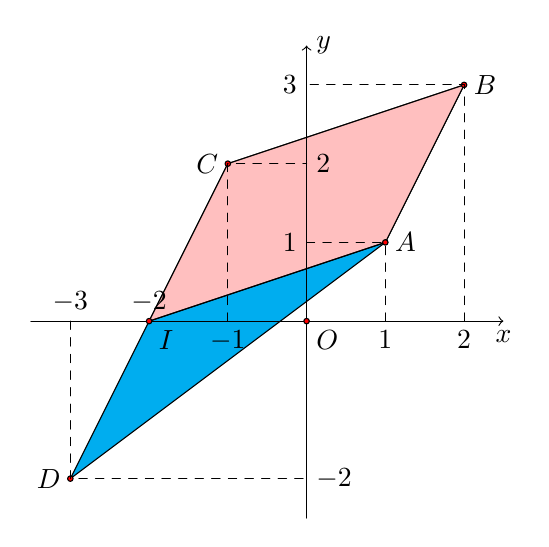
\begin{tikzpicture}[scale=1, line join=round, line cap=round]
			\coordinate (O) at (0,0);
			\coordinate (A) at (1,1);
			\coordinate (B) at (2,3);
			\coordinate (C) at (-1,2);
			\coordinate (I) at (-2,0);
			\coordinate (D) at (-3,-2);
			\draw[fill=cyan] (A)--(B)--(C)--(D)--cycle;
			\draw[fill=pink] (A)--(B)--(C)--(I)--cycle;
			\draw[->] (-3.5,0)--(2.5,0) node [below]{$x$};
			\draw[->] (0,-2.5)--(0,3.5) node [right]{$y$};	
			\draw (I)--(A);
			\foreach \x in {A,B,C,D,I,O}{\draw[fill=red] (\x) circle (1pt);
			}
			\foreach \x in {A,B}{\draw (\x) node[right]{$\x$};}
			\foreach \x in {C,D}{\draw (\x) node[left]{$\x$};}
			\foreach \x in {I,O}{\draw (\x) node[below right]{$\x$};}
			\draw[dashed] (-3,0)--(D)--(0,-2) (-1,0)--(C)--(0,2) (1,0)--(A)--(0,1) (2,0)--(B)--(0,3);
			\draw (-3,0) node[above]{$-3$};
			\draw (-2,0) node[above]{$-2$};
			\foreach \x in{-1,1,2} \draw (\x,0) node[below]{$\x$};
			\foreach \x in{1,3} \draw (0,\x) node[left]{$\x$};
			\foreach \x in{2,-2} \draw (0,\x) node[right]{$\x$};
%			\draw[line width=0.1pt,dashed] (-3.5,-2.5) grid (2.5,3.5);
		\end{tikzpicture}}
	\item \immini{Lấy điểm $A'$ đối xứng với $A$ qua $B$. Ta có $\vec{AB}=\vec{BA'}$.\\
	Lúc đó $\vec{CB}+\vec{AB}=\vec{CB}+\vec{BA'}=\vec{CA'}$.\\
	Suy ra $|\vec{CB}+\vec{AB}|=|\vec{CA'}|=CA'$.\\
	Theo định lí Pytago ta có
	\begin{eqnarray*}
		A'C&=&\sqrt{AC^2+AA'^2}\\
		&=&\sqrt{(3a)^2+(4a)^2}=5a.
	\end{eqnarray*}}{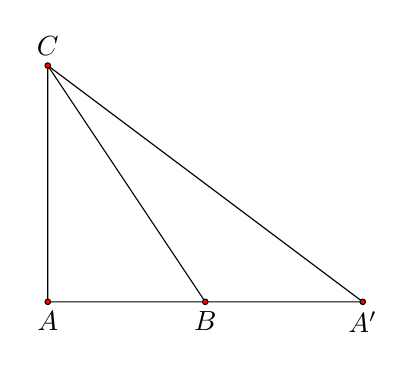
\begin{tikzpicture}[scale=1, line join=round, line cap=round]
	\coordinate (A) at (0,0);
	\coordinate (B) at (2,0);
	\coordinate (A') at (4,0);
	\coordinate (C) at (0,3);
	\draw (A)--(A')--(C)--cycle; 
	\draw (C)--(B);
	\foreach \x in {A,B,C,A'}{\draw[fill=red] (\x) circle (1pt);}
	\foreach \x in {A,B,A'}{\draw (\x) node[below]{$\x$};}
	\draw (C) node[above]{$C$};
\end{tikzpicture}}

	\end{enumerate}
		
}
\end{bt}

\begin{bt}%[0H2G3-5]%[0D2K2-3]%[Dự án đề kiểm tra HKII NH22-23- Huỳnh Quy]%[Tên TrườngTHPT Chuyên Nguyễn Tất Thành - Yên Bái]
	\begin{enumerate}
		\item Cho tam giác $ABC$. Kẻ đường phân giác $AM$ ($M$ thuộc cạnh $BC$). Đặt $AB=c$, $AC=b$. Chứng minh rằng $\vec{AM}=\dfrac{b}{b+c}\vec{AB}+\dfrac{c}{b+c}\vec{AC}$.
		\item Bạn An có $48$g bột nho và $240$g đường. An muốn pha chế thành hai loại nước nho A và B để bán trong một sự kiện gây quỹ cho lớp. Để pha chế $1$ lít nước nho loại A cần $30$g đường và $4$g bột nho; pha chế $1$ lít nước nho loại B cần $20$g đường và $8$g bột nho. Mỗi lít nước nho loại A bán lãi $40$ nghìn đồng, mỗi lít nước nho loại B bán lãi $60$ nghìn đồng. Hỏi bạn An nên pha chế bao nhiêu lít nước nho mỗi loại để thu được lợi nhuận cao nhất?
	\end{enumerate}
\loigiai{
	\begin{enumerate}
		\item Ta có $AM$ là phân giác của của góc $\widehat{A}$ nên ta có 
		\begin{eqnarray*}
			&&\dfrac{BM}{c}=\dfrac{MC}{b}=\dfrac{BM+MC}{b+c}=\dfrac{BC}{b+c}\\
			&\Rightarrow&\dfrac{BM}{BC}=\dfrac{c}{b+c}\\
			&\Rightarrow&\vec{BM}=\dfrac{c}{b+c}\vec{BC}\quad(\text{vì}\, \vec{BM}\,\text{và}\, \vec{BC}\, \text{cùng hướng})
		\end{eqnarray*}
	Do đó:\allowdisplaybreaks
	\begin{eqnarray*}
		\vec{AM}&=&\vec{AB}+\vec{BM}\\
		&=&\vec{AB}+\dfrac{c}{b+c}\vec{BC}\\
		&=&\vec{AB}+\dfrac{c}{b+c}(\vec{AC}-\vec{AB})\\
		&=&\left(1-\dfrac{c}{b+c}\right)\vec{AB}+\dfrac{c}{b+c}\vec{AC}\\
		&=&\dfrac{b}{b+c}\vec{AB}+\dfrac{c}{b+c}\vec{AC}\quad(\text{đpcm}).
	\end{eqnarray*}
	\item Gọi $x$, $y$ lần lượt là số lít nước nho loại A và B cần pha chế ($x,y\ge 0$).\\
	Số gam bột nho cần dùng là $4x+8y\le 48$.\\
	Số gam đường cần dùng là $30x+20y\leq 240$.\\
	Lợi nhuận thu được là $F(x;y)=40x+60y$ (nghìn đồng).\\
	Ta cần tìm $x$, $y$ để $F(x;y)$ lớn nhất.\\
	Ta có $\heva{&x,y\geq 0\\&4x+8y\le 48\\&30x+20y\leq 240}\Leftrightarrow\heva{&x,y\geq 0\\&x+2y\leq 12\\&3x+2y\leq 24.}$\\
	Biểu diễn miền nghiệm của hệ bất phương trình lên mặt phẳng tọa độ:
	\begin{center}
		\begin{tikzpicture}[font=\footnotesize,line join=round, line cap=round, >=stealth,scale=0.8] 
			\def \xmin{-1}\def \xmax{9}\def \ymin{-1}\def \ymax{7} 
			\draw[->] (\xmin,0)--(\xmax+0.2,0) node[shift=(-90:0.25)] {$x$};
			\draw[->] (0,\ymin)--(0,\ymax+0.2) node[shift=(0:0.25)] {$y$};
			\fill (0,0) circle(1pt) node[shift=(45:0.25)]{$O$}
			(6,0) circle(1pt) node[shift=(-90:0.2)]{$6$}
			(8,0) circle(1pt) node[shift=(-90:0.2)]{$8$}
			(0,3) circle(1pt) node[shift=(180:0.2)]{$3$}
			(0,6) circle(1pt) node[shift=(180:0.2)]{$6$}
			(0,6) circle(1pt) node[shift=(-55:0.45)]{$A$}
			(6,3) circle(1pt) node[shift=(-120:0.25)]{$B$}
			(8,0) circle(1pt) node[shift=(150:0.4)]{$C$};
			\begin{scope}
				\clip (\xmin,\ymin) rectangle (\xmax,\ymax); 
				\draw[smooth,samples=100,domain=\xmin:\xmax] plot(\x,{6-0.5*\x});
				\draw[smooth,samples=100,domain=\xmin:\xmax] plot(\x,{12-1.5*\x});
				\fill[pattern=north east lines,opacity=.8] plot[domain=\xmin:\xmax] (\x,{6-0.5*\x})--(\xmax,\ymin)--(\xmax,\ymax)--(\xmin,\ymax)--cycle;
				\fill[pattern=north west lines,opacity=.8] plot[domain=\xmin:\xmax] (\x,{12-1.5*\x})--(\xmax,\ymin)--(\xmax,\ymax)--(\xmin,\ymax)--cycle;
				\fill[pattern=north west lines,opacity=.8] (\xmin,\ymax)--(0,\ymax)--(0,\ymin)--(\xmin,\ymin)--cycle;
				\fill[pattern=north east lines,opacity=.8] (\xmin,\ymin)--(\xmin,0)--(\xmax,0)--(\xmax,\ymin)--cycle;
			\end{scope}
			\draw[dashed] (0,3)--(6,3)--(6,0);
		\end{tikzpicture}
	\end{center}
	Miền nghiệm của hệ bất phương trình là đa giác $OABC$ với $O(0;0)$, $A(0;6)$, $B(6;3)$, $C(8;0)$.\\
	Ta có $F(0;0)=0$, $F(0;6)=360$ nghìn đồng; $F(6;3)=420$ nghìn đồng, $F(8;0)=320$ nghìn đồng.\\
	Ta có $F(x;y)$ đạt giá trị lớn nhất khi $\heva{&x=6\\&y=3.}$\\
	Vậy cần pha chế $6$ lít nước nho loại A và $3$ lít nước nho loại B để lợi nhuận thu được là lớn nhất.
	\end{enumerate}
}
\end{bt}


\begin{center}
	\textit{Phần B}
\end{center}

\begin{bt}%[0X1Y3-1]%[0X1Y4-3]
Kết quả dự báo nhiệt độ cao nhất trong 10 ngày liên tiếp từ 30/12/2022 đến 8/1/2023 tại SaPa được cho trong bảng sau (\textit{https://thoitiet.vn}):
\begin{center}
	\begin{tabular}{|c|c|c|c|c|c|c|c|c|c|c|}
\hline
Ngày/tháng &30/12&31/12&1/1&2/1&3/1&4/1&5/1&6/1&7/1&8/1 \\
\hline
Nhiệt độ ($^\circ C$)& 5 & 6 & 8 & 9 & 8 & 11 & 11 & 12 & 11 & 12 \\
\hline
\end{tabular}
\end{center}
\begin{enumerate}
\item Tính số trung bình và khoảng biến thiên nhiệt độ cao nhất trong 10 ngày liên tiếp tại SaPa được cho trong bảng trên.
\item Tính phương sai và độ lệch chuẩn cho mẫu số liệu này.
\end{enumerate}
\loigiai{
Ta có bảng tần số của mẫu số liệu 
\begin{center}
\begin{tabular}{|c|c|c|c|c|c|c|}
\hline
Nhiệt độ($^\circ C$)&5&6&8&9&11&12\\
\hline
Số ngày&1&1&2&1&3&2\\
\hline
\end{tabular}
\end{center}
\begin{enumerate}
\item Nhiệt độ trung bình tại SaPa trong 10 ngày liên tiếp\[\overline{x}=\dfrac{5\cdot 1+6\cdot 1+8\cdot 2+9\cdot 1+11\cdot 3+12\cdot 2}{10}=9{,}3^\circ C.\]
\item 
Phương sai của mẫu số liệu
\begin{eqnarray*}
S^2&=&\dfrac{1}{10}\left[\foreach\x in {5,6,8,9,11}{(\x-9{,}3)^2+}(12-9{,}3)^2\right]\\
&\approx&6{,}23.
\end{eqnarray*}
Độ lệch chuẩn của mẫu số liệu
\[\sigma=\sqrt{S^2}\approx2{,}5.\]
\end{enumerate}
}
\end{bt}
\begin{bt}%[0H4Y1-6]%[0H4K1-6]
\begin{enumerate}
\item Trên mặt phẳng tọa độ $O x y$ cho 3 điểm không thẳng hàng $A(1 ; 1)$, $B(2 ; 3)$, $C(-1 ; 2)$. Tìm tọa độ điểm $D$ sao cho tứ giác $A B C D$ là một hình bình hành.
\item Cho tam giác $A B C$ vuông tại $A$ và $A B=3 a$, $A C=2 a$. Tính độ dài của vectơ $\overrightarrow{B C}+\overrightarrow{A C}$.
\end{enumerate}
\loigiai{
\begin{enumerate}
\item Gọi $D(x;y)$ là tọa độ điểm cần tìm.\\
Ta có $\overrightarrow{AB}=(1;2)$, $\overrightarrow{DC}=(-1-x;2-y)$.\\
Vì $ABCD$ là hình bình hành\\
Nên $\overrightarrow{AB}=\overrightarrow{DC}\Leftrightarrow \heva{&-1-x=1\\&2-y=2}\Leftrightarrow\heva{&x=-2\\&y=0.}$\\
Vậy $D(-2;0)$.
\item~
\begin{center}
\begin{tikzpicture}
	\path (0,0) coordinate (A)
	(6,0) coordinate (B)
	(0,4) coordinate (C)
	($(A)!.5!(B)$) coordinate (M);
	\draw (A)--(B)--(C)--cycle (C)--(M);
	\pic[draw,angle radius=8pt]{right angle=C--A--M};
	\foreach \t/\g in {A/-135,B/-90,C/90,M/-90}{
		\draw[fill=white] (\t) circle (1pt) node[shift={(\g:7pt)},font=\scriptsize]{$ \t $};
	}
\end{tikzpicture}
\end{center}
Gọi $M$ là trung điểm của $AB$. Suy ra $AM=MB=1{,}5a$.\\
Ta có
\begin{eqnarray*}
\overrightarrow{BC}+\overrightarrow{AC}=-\left(\overrightarrow{CA}+\overrightarrow{CB}\right)=-2\overrightarrow{CM}\Rightarrow \left|\overrightarrow{BC}+\overrightarrow{AC}\right|=2|\overrightarrow{CM}|=2CM.
\end{eqnarray*}
$\triangle ACM$ vuông tại $A$ nên $CM=\sqrt{AM^2+AC^2}=\sqrt{(1{,}5a)^2+(2a)^2}=\dfrac{5}{2}a$.\\
Vậy $\left|\overrightarrow{BC}+\overrightarrow{AC}\right|=\dfrac{5}{2}a$.
\end{enumerate}
}
\end{bt}
\begin{bt}%[0D2K2-3]
\begin{enumerate}
\item Trên mặt phẳng tọa độ $O x y$ cho hai điểm $A(1 ;-3), B(5 ; 1)$. Tìm tọa độ điểm $M$ thuộc trục $O x$ sao cho độ dài $M A+M B$ là ngắn nhất.
\item Bạn An có $48 g$ bột nho và $240 g$ đường. An muốn pha chế thành hai loại nước nho $A$ và $B$ để bán trong một sự kiện gây quỹ cho lớp. Để pha chế 1 lít nước nho loại $A$ cần $30 g$ đường và $4 g$ bột nho; pha chế 1 lít nước nho loại $B$ cần $20 g$ đường và $8 g$ bột nho. Mỗi lít nước nho loại $A$ bán lãi $40$ nghìn đồng, mỗi lít nước nho loại $B$ bán lãi 60 nghìn đồng. Hỏi bạn An nên pha chế bao nhiêu lít nước nho mỗi loại để thu được lợi nhuận cao nhất?
\end{enumerate}
\loigiai{
\begin{enumerate}
\item
\textbf{Nhận xét:} Hai điểm $A(1;-3)$ và $B(5;1)$ nằm khác phía với trục $Ox$.
\immini{
Dựa vào hình vẽ bên, áp dụng bất đẳng thức tam giác, ta có $MA+MB\geq AB$.\\
Dấu ``$=$'' xảy ra khi $M$, $A$, $B$ thẳng hàng. Khi đó $M$ là giao điểm của đường  $AB$ và trục $Ox$.\\
Ta có $\overrightarrow{AB}=(4;4)$. Suy ra đường thẳng $AB$ có một véc-tơ pháp tuyến là $\vec{n}=(1;-1)$.\\
Phương trình tổng quát của đường thẳng $AB$ là 
\[(AB)\colon 1\cdot (x-1)-1\cdot (y+3)=0\Leftrightarrow (AB)\colon x-y-4=0.\]
Với $y=0$, thì $x=4$.\\
Vậy $M(4;0)$ là điểm cần tìm.
}
{\begin{tikzpicture}[>=stealth,font=\footnotesize]
		\draw[->] (-1,0)--(5,0) node[above]{$x$};
		\draw[->] (0,-4)--(0,3) node[right]{$y$};
		\path (0,0) coordinate (O)
		(1,-3)  coordinate (A)
		(5,1) coordinate (B)
		(3,0) coordinate (M)
		;
		\draw (A)--(B)--(M)--cycle;
		\foreach \t/\g in {A/-45,B/90,O/-45,M/90}{
			\fill (\t) circle (1pt) node[shift={(\g:7pt)}]{$ \t $};
		}
\end{tikzpicture}}
\item Gọi $x$, $y$ lần lượt là số lít nước nho loại $A$, $B$ ($x,y>0$).
\immini{Theo đề bài ta có hệ bất phương trình\\
$\heva{&30x+20y\leq 240\\&4x+8y\leq48}\Leftrightarrow\heva{&3x+2y\leq 24\\&x+2y\leq 12&}$\tagEX{$*$}
Miền nghiệm của hệ bất phương trình $(*)$ là tứ giác $OABC$ với $A(8;0)$, $B(6;3)$, $C(0;6)$.\\
Lợi nhuận An thu được là  $F(x;y)=40x+60y$.\\
Ta có
\begin{itemize}
	\item $F(0;0)=0$;
	\item $F(8;0)=320$;
	\item $F(6;3)=420$;
	\item $F(0;6)=360$.
\end{itemize}
Vậy để thu được lợi nhuận nhiều nhất thì An cần làm $6$ lít nước cam loại $A$ và $3$ lít nước cam loại $B$.
}
{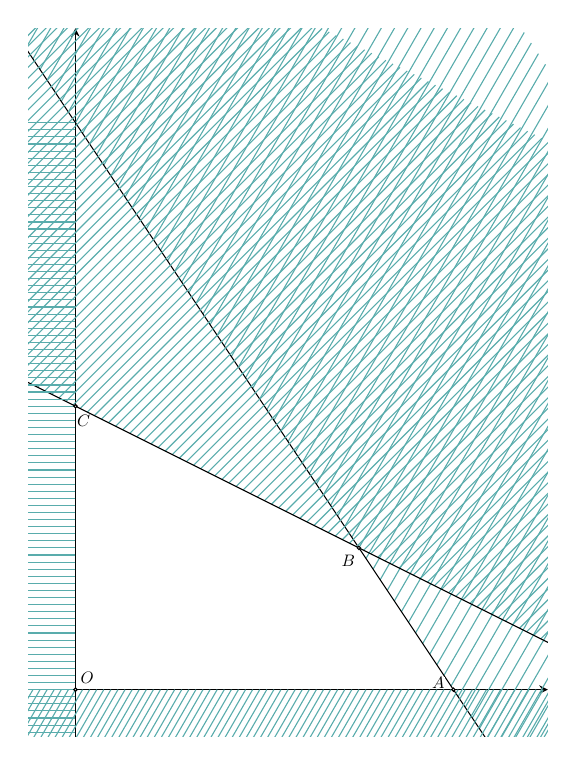
\begin{tikzpicture}[>=stealth,smooth,samples=100,transform shape,scale=0.6]
		\draw[->] (-1,0)--(10,0);
		\draw[->] (0,-1)--(0,14);
		\begin{scope}
			\clip (-1,-1) rectangle (10,14);
			\foreach \i in {-12,-11.85,...,12}{
				\draw[teal!65,thin]({\i},{(-3*\i--24)/2})--+(60:10);}
			\draw plot[domain=-10:10]({\x},{(-3*\x--24)/2});
			\foreach \i in {-8,-7.85,...,21}{
				\draw[teal!65,thin]({\i},{(-1*\i--12)/2})--+(45:10);}
			\draw plot[domain=-6:15]({\x},{(-1*\x--12)/2});
			\foreach \i in {-12,-11.85,...,12}{
				\draw[thin,teal!65]({-(0)},{\i})--+(180:10);}
			\foreach \i in {-12,-11.85,...,12}{
				\draw[teal!65,thin]({\i},{(-0*\i-0)/1})--+(-120:10);}
		\end{scope}
		\path (0,0) coordinate (O)
		(8,0) coordinate (A)
		(6,3) coordinate (B)
		(0,6) coordinate (C);
		\foreach\x/\y in{A/155,B/-130,C/-60,O/45}{\draw[fill=white] (\x) circle (1pt)node[shift={(\y:.35)},fill=white,inner sep=0pt]{$\x$};}
\end{tikzpicture}}
\end{enumerate}
}
\end{bt}
